\documentclass[../../main/thesis_msc.tex]{subfiles}



\begin{document}

    \chapter{Introduction}
    
		The cycle of life and death of stars  baffled astronomers for many years. The study of stellar structure and evolution continues -up to this date- to be of paramount importance, since it is crucial to our understanding of various branches of astronomy, e.g. the structure of galaxies, and chemical history of the Universe.
		
		The aim of this thesis is to investigate and get an insight in one of the most debated topics in Stellar Astrophysics; the connection between the progenitor and remnant masses, especially in the case of double neutron star binary systems. The existence of those systems was recently confirmed by the detection of gravitational waves emitted during a merging event, accompanied by the detection of a kilonova -the "afterglow"of such an event- as described in the seminal paper of the LIGO/VIRGO collaborations \citep{ligo}.
		
		In this chapter, a synopsis that extends from the formation to the death of helium stars will be attempted. A detailed coverage of the principles of stellar evolution is beyond the scope of this thesis and a fundamental knowledge is assumed. Moreover, for the interested reader, there are classical textbooks \citep{Kipp_book, Clayton, Prialnik, Eggleton_book} covering almost every aspect in the field of stellar astrophysics. Nevertheless, for the sake of completeness, a small introduction to several fundamental notions, tailored to our needs, will also be carried out in the next few pages. 
		

    
    
    \section{Helium stars}
    	
    	%A brief explanation of what a helium star is
    	From the large primordial molecular clouds, protostars are being constantly formed via a process called \emph{gravoturbulent cloud fragmentation}. When the accretion of the surrounding material from the protostellar core ceases, the protostar is said to be in the \emph{pre-main sequence} (PMS) phase of its evolution, and continues to contract under the force of gravity until the central temperature becomes sufficiently high for nuclear fusion reactions on hydrogen to occur. At this point, the star enters the \emph{main sequence} (MS) evolutionary phase as a zero-age main sequence (ZAMS) star where it will spend most of its life.
    	
    	During the MS stage, the star converts hydrogen to helium either via the pp-chain reactions, or via the CNO cycles, depending on its initial mass and chemical composition. Slowly but steadily, the hydrogen in the core is being consumed by the aforementioned nuclear networks, and helium builds up forming a helium core. This process continues until the hydrogen in the stellar core is depleted, resulting to an inert hydrogen envelope engulfing the newly formed He-core; subsequently, the star exits the MS phase and the nuclear reactions in its interior that provided the necessary pressure support against gravity, effectively stop. Since the star is not in an equilibrium state anymore, it starts to contract until hydrogen is ignited in a shell around the inert helium core. At this point, the star enters the so-called \emph{red-giant branch} (RGB) and the hydrogen-rich envelope, on top of the H-burning shell, inflates rapidly whilst the He-core continues to contract due to the \emph{mirror principle} \citep[see][p.~369]{Kipp_book}.
    	
    	As we will explain in a moment, the hydrogen envelope can be lost when the star is in the RGB phase, with more than one ways, exposing the He-core of the star. This naked, hydrogen deficient, He-core is what we refer to as a \emph{helium star}. We can classify He-stars into two groups: low-mass \emph{hot subdwarfs} (sd) that can be further subdivided into several categories (e.g. sdB, sdO) based on their spectra, and more massive \emph{Wolf-Rayet} (WR) stars that can also be subdivided into several classes (e.g. WN, WC). For a more detailed discussion we refer the reader to the work of \cite{Han2002, Han2003, Heber2009, Chiosi86, langer12}.


			\subsection{Formation of helium stars}
			
				%A small section explaining how helium stars are being formed
				Helium stars can be formed either in isolation or as part of a binary system. In both scenarios, the physical mechanism that is responsible for the stripping of the hydrogen envelope is of the utmost importance.
				
				In the former case of a single He-star, the necessary mass loss is being achieved due to strong, radiation-driven, stellar winds. However, the specifics of such a process have not been fully resolved yet, and an enhanced mass loss scheme, e.g. caused by rotational mixing, magnetic fields, or even strong He-flashes should be considered for the progenitor of the He-star \citep{Sweigart, Heber2009}. 
				
				In the case where the He-star progenitor is part of a binary system, the required strong mass loss can be achieved via different channels, depending on how wide the binary system is. These channels include the stable Roche-lobe overflow (RLO) and the Common Envelope (CE) ejection. We will discuss these mass loss mechanisms below.
				It should be mentioned that sdB stars can also originate from the merging of two helium white dwarfs (He-WD) in a close binary, resulting to an object with enough mass to ignite helium \citep{Han2002}.
				
				
			
			\subsection{Evolution of single helium stars}
			
				%A small section explaining the evolution of single helium stars 
				Once the He-star progenitor has been stripped from its hydrogen envelope during the RGB phase, the compression of the core continues until it reaches the necessary conditions for helium to ignite at its centre. The ignition of core helium burning signifies the transition to the helium main sequence (He-MS) as a He-ZAMS star. The last two concepts are defined in a similar way to the (hydrogen) main sequence and ZAMS respectively.
				
				During the He-MS stage, the star burns its $^4$He supply via the triple-alpha process producing carbon ($^{12}$C) and the stable oxygen isotope $^{16}$O, as a byproduct. When the helium in the core is depleted, the contraction/expansion process we described above is repeated; the idle metal core that has been formed, consists mainly of carbon, oxygen, neon, and magnesium and it is surrounded by a He-rich envelope. This whole structure will contract until helium is ignited in a shell at the bottom of the envelope, followed by the ignition of carbon in the centre (given that the star is massive enough). The fate of the He-star at this point depends on its mass; if it has not retain enough mass for carbon ignition, it will gradually cool off and end its life as a carbon/oxygen white dwarf (CO WD). On the other hand, if it is massive enough to ignite carbon, either on or off centre, its fate could be an oxygen/neon/magnesium white dwarf (ONeMg WD), a hybrid white dwarf (CONeMg WD), or even collapse as a supernova.
				
				\begin{figure}[t]
					\centering
					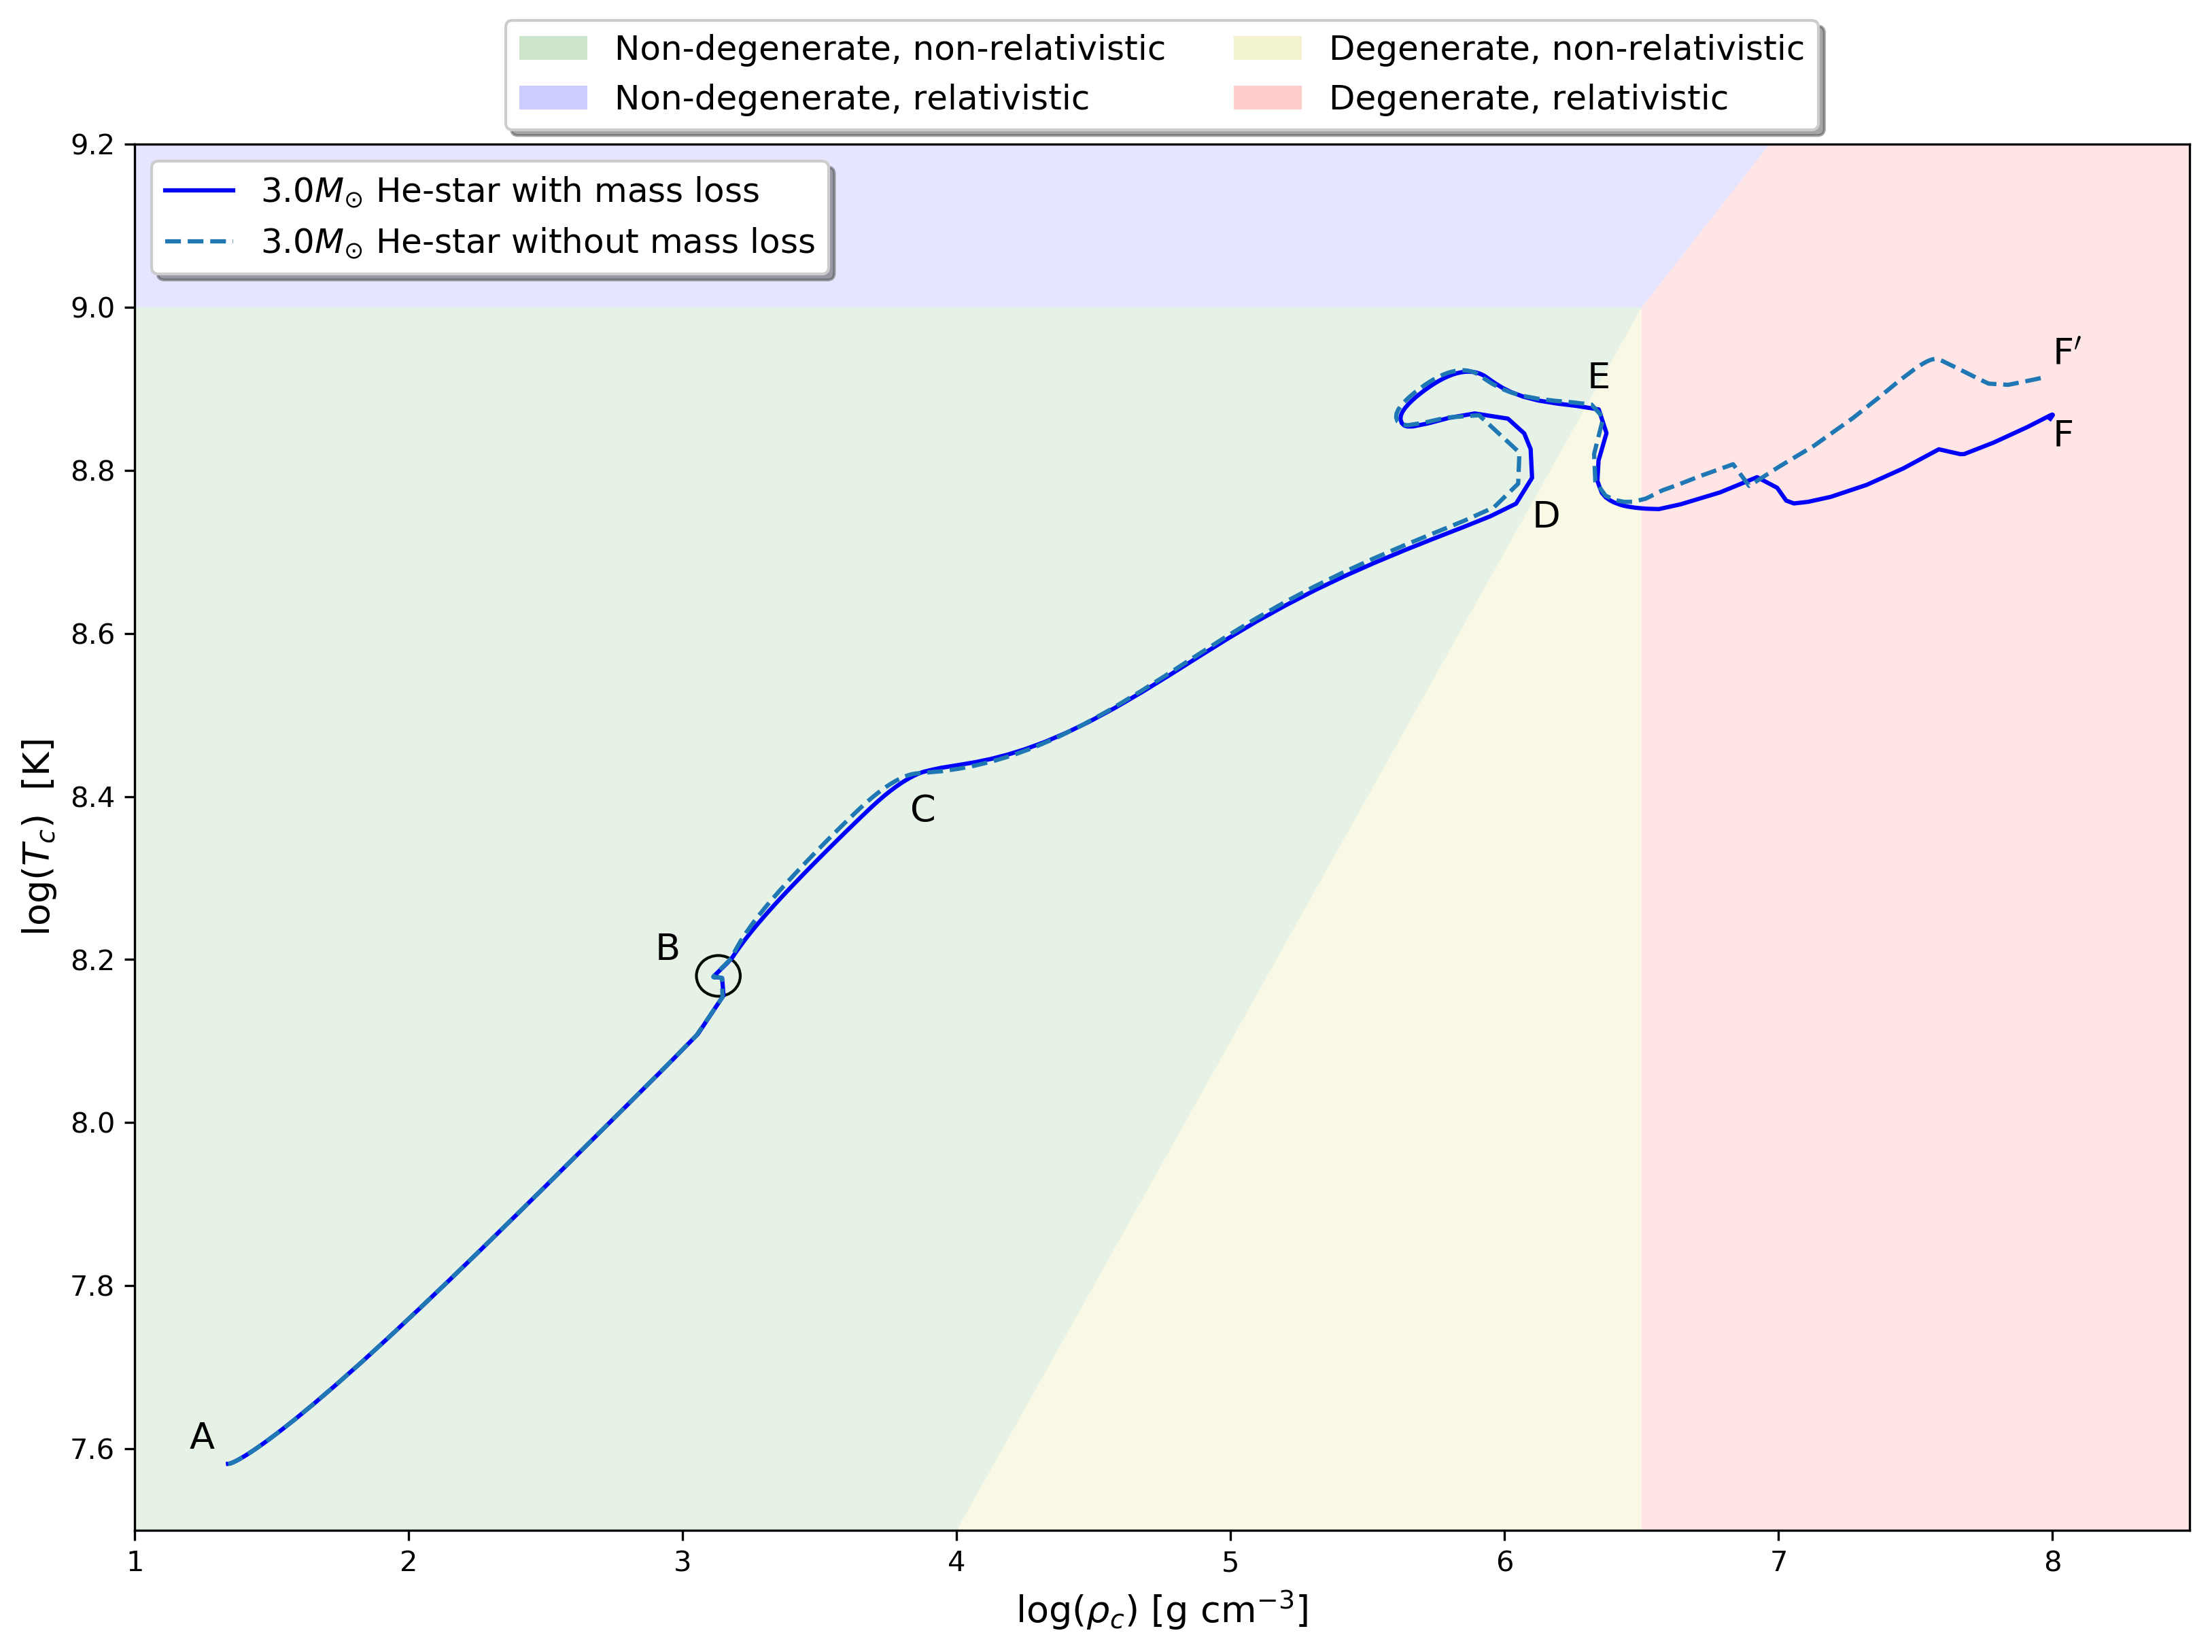
\includegraphics[scale=0.5]{../figures/chapter1/T_rho_plane_ch1_shaded.png}
					\caption{The evolution of a $3.0$ M$_{\odot}$ He-star, with and without mass loss. The point where the star enters the He-MS as a He-ZAMS can be seen as a small hook inside the black circle. An analytic explanation of the letters along the evolutionary tracks, is provided in the text. The coloured areas illustrate the different regimes of pressure.}
					\label{fig:T_rho_plane_ch1}
				\end{figure}
				
				To demonstrate the aforementioned stages, the evolutionary track of a $3.0$ M$_{\odot}$ He-star (with and without mass loss) is illustrated in the $T_c - \rho_c$ plane (\hyperref[fig:T_rho_plane_ch1]{Fig 1.1}) \citep[see also][]{Habets_a, Habets_b, Nomoto1987}. The letters denote the beginning and end of several phases up to the off-centre neon ignition. The A-B phase shows the contraction that follows after the RGB stage of the progenitor. The moment of core He-ignition is denoted by the black circle at point B, and marks the entrance to the He-MS phase (B-C). At point C, helium has been exhausted and the core contracts whilst He-shell burning follows. During the D-E phase, the carbon is ignited in the core making a loop in the diagram around $\rho_c = 10^6$ g cm$^{-3}$. Finally, the E-F/F$^\prime$ shows the carbon-shell burning along the contraction of the O-Ne-Mg core; at the endpoint (F/F$^\prime$), neon is ignited off-centre.
				
				Conveniently, in the same figure one can see the approximate regimes of pressure which are illustrated as coloured regions. For the conditions in the green area, the stellar material is non-degenerate and non-relativistic hence the dominant pressure can be approximated by the ideal gas law ($P_{\text{gas}}$). The blue area shows the region where the gas is still in a non-degenerate state but the temperature is so high that forces the electrons to move with speeds that are comparable to the speed of light. Under these conditions, the pressure provided by the exerted radiation ($P_{\text{rad}}$) begins to dominate over the gas pressure. Moving to higher densities the electron gas becomes degenerate, first non-relativistically (yellow area) and then relativistically (red area). In both cases the pressure is provided by the degenerate electron gas. From the diagram it becomes clear that degeneracy can be lifted if the temperature is sufficiently high.
				
				These boundaries for the pressure regimes can be easily found if we equate the relevant expressions of pressure given by the equation of states for each regime (e.g. $P_{\text{gas}} = P_{\text{rad}}$, for the two non-degenerate regions). In reality the transition among the different regimes is continuous and not sharp as depicted here, which can be misleading. Nevertheless, this way of imaging provides us with a visual aid of where in the evolutionary stage of a star relativistic, or quantum mechanical effects can be of great importance.
				
				\begin{comment}
				For a more complete and comprehensive overview of the evolution of single He-stars, we provide, in the form of a Kippenhahn diagram, the net energy production rate with respect to the internal structure of the $3.0$ M$_{\odot}$ star (with mass loss) we used in the example above (\hyperref[fig:Kipp_3p0_ch1]{Fig 1.2}). In this diagram, the x-axis expresses the remaining time of the calculations whilst the y-axis shows the inner structure of the star in terms of mass coordinates. The color scale is associated with the energy production.
				
				\begin{figure}[h]
					\centering
					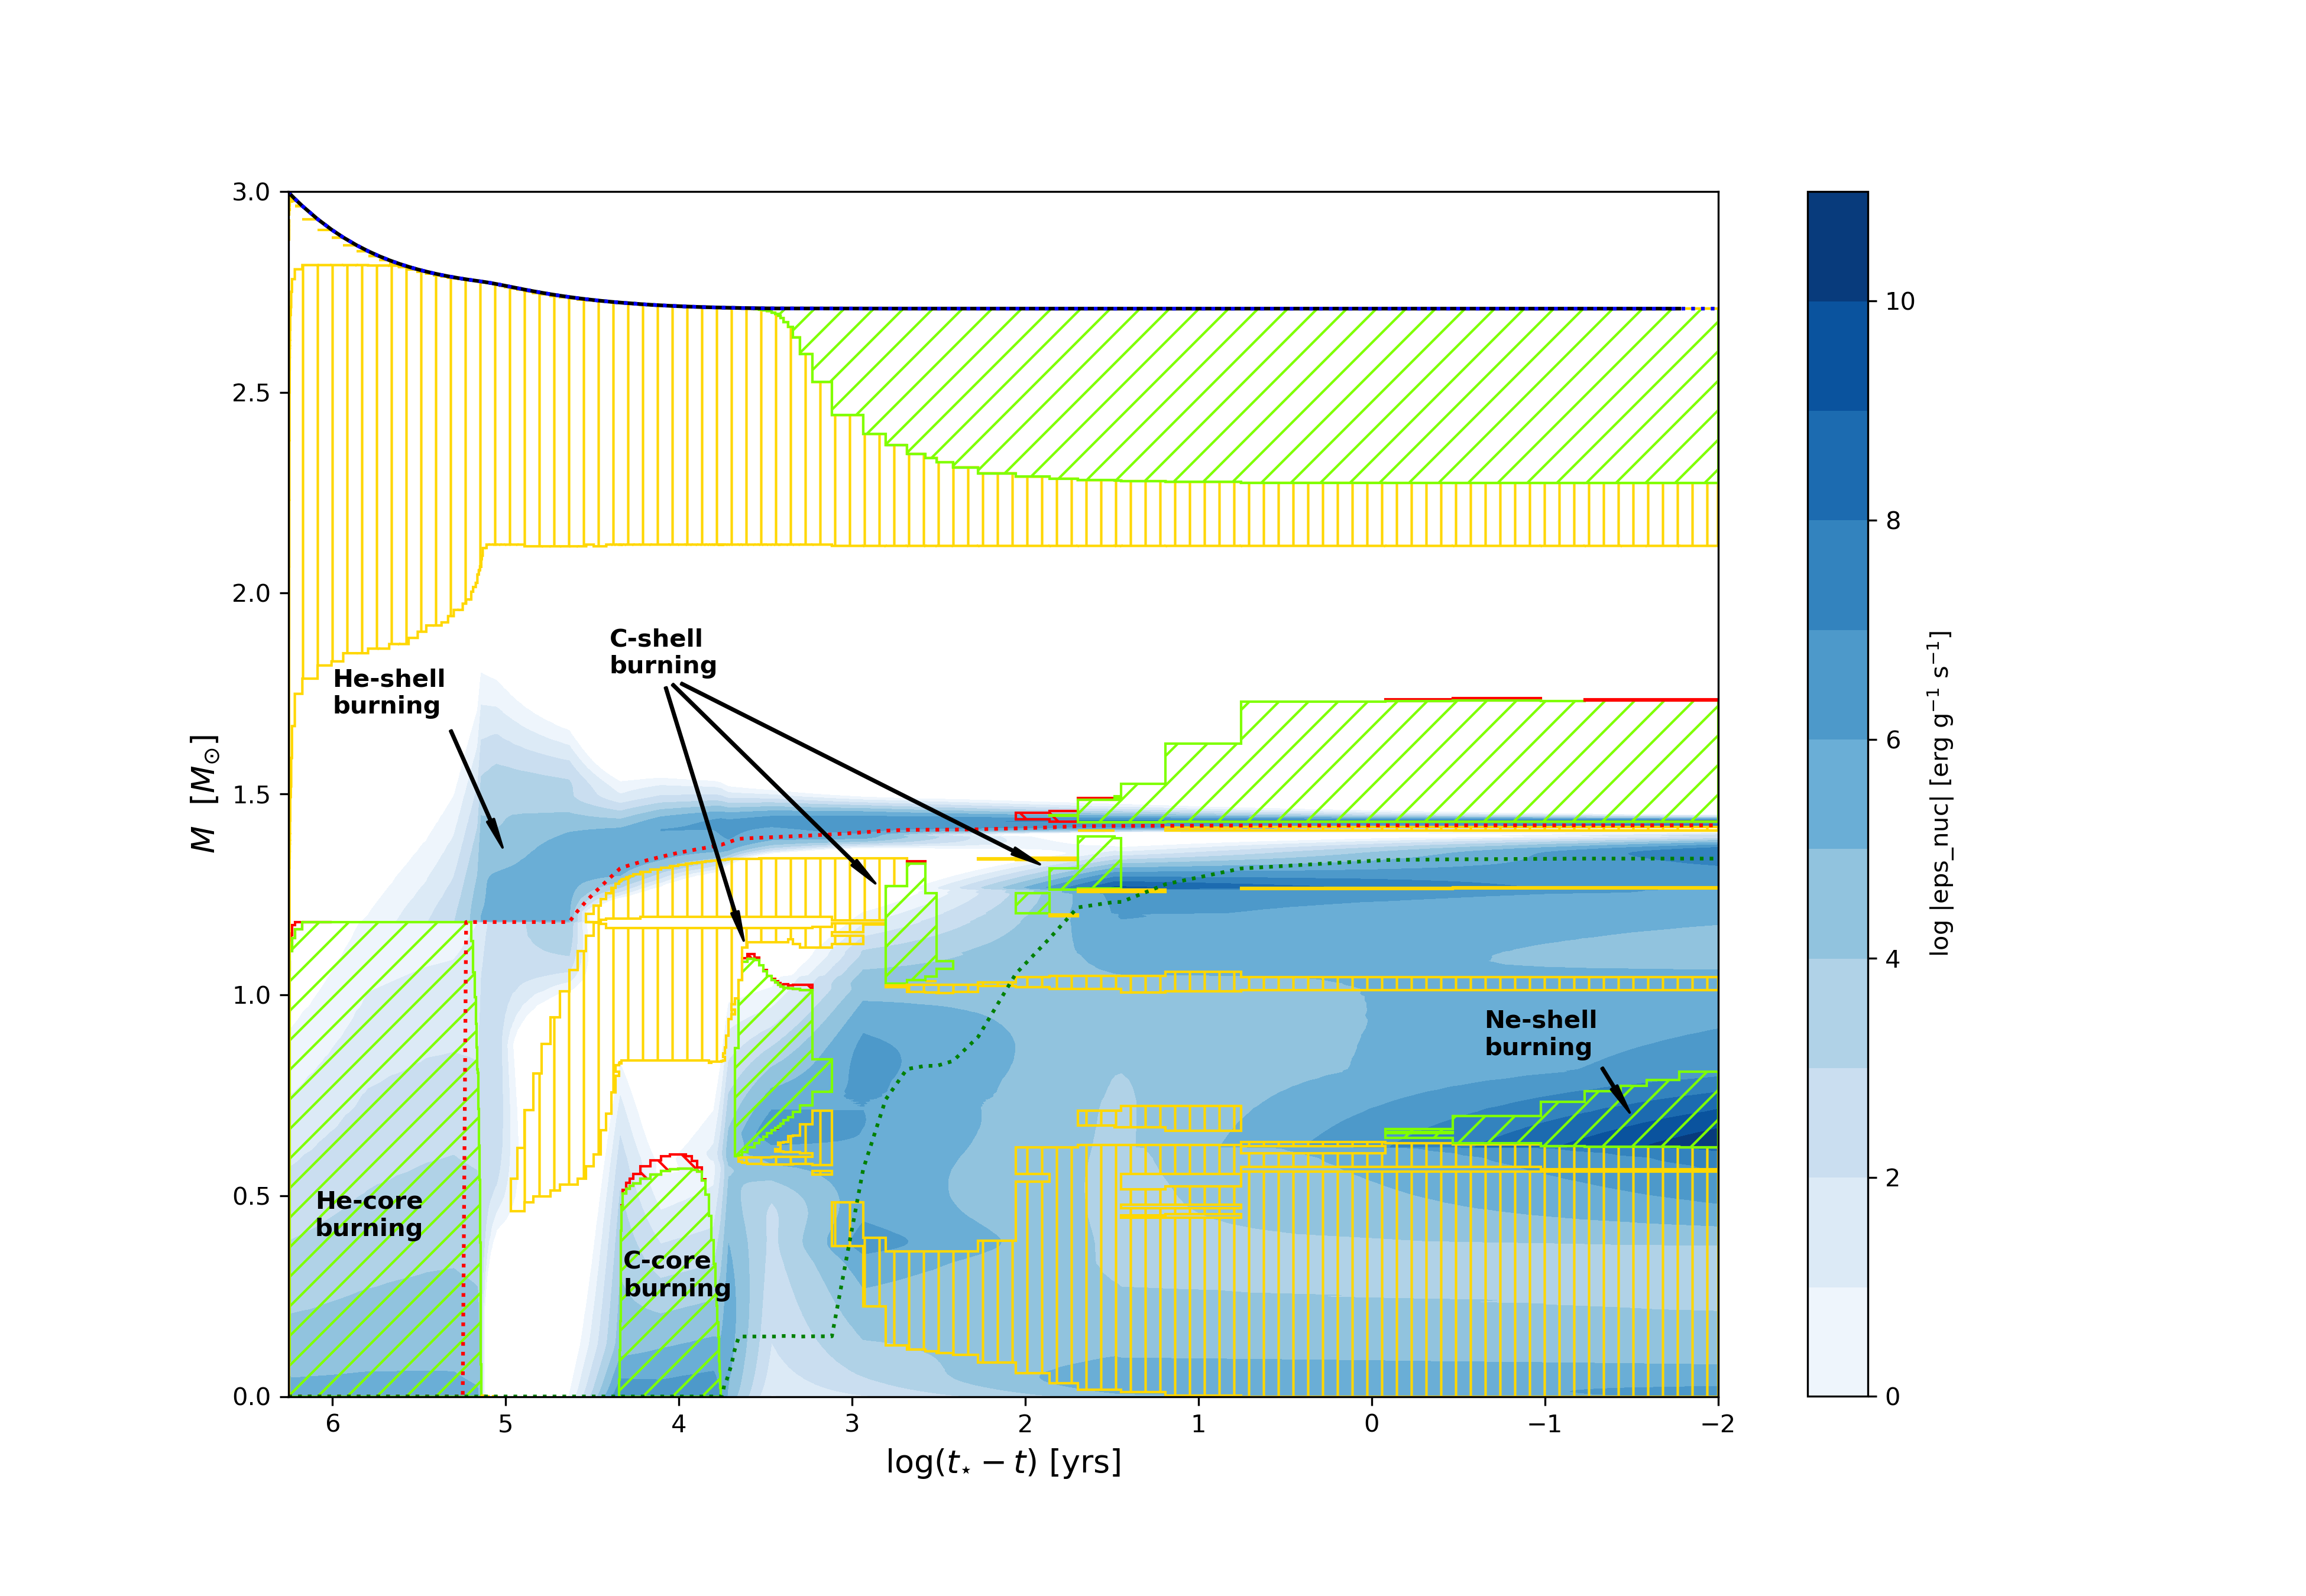
\includegraphics[width=\textwidth]{../figures/chapter1/Kippenhahn_intro.png}
					\caption{Kippenhahn diagramm for a $3.0$ M$_{\odot}$ He-star with mass loss. The green and gold hatched areas denote convective and thermohaline mixing respectively. Red solid lines represent areas with semi-convective mixing. The black, red, and green dotted lines show the build-up of helium, carbon, and oxygen core mass respectively.}
					\label{fig:Kipp_3p0_ch1}
				\end{figure}
				
				By taking a careful look at \hyperref[fig:Kipp_3p0_ch1]{Fig 1.2}, we observe that during He-burning in the convective core, the star experiences an approximately $\sim 0.3$ M$_{\odot}$ mass loss via stellar winds. As a result of this core burning process, a C-core of $\sim 1.2$ M$_{\odot}$ is formed that continues to grow up to $\sim 1.42$ M$_{\odot}$ due to He-shell burning. Similarly, an oxygen core is formed of about $\sim 1.34$ M$_{\odot}$ as a result of the more advanced burning stages.
				\end{comment}
				
				
				
				
				
				
					\subsubsection{Mixing mechanisms}
					
						%convection, overshooting, thermohaline
						Although protostars begin their life with, a more or less, uniform elemental composition which is the same as the composition of the cloud they originated from, the ongoing nuclear reactions transform and create new elements that are not necessarily distributed uniformly throughout the stellar interior. This is because there are several ways for a star to stir and mix its material. These mixing mechanisms are usually caused by various instabilities and can contribute on different levels based on specific conditions. In this section we will briefly explain four major mixing processes leaving the effects of rotation for later discussion.
						
						Maybe the most effective way to transfer material is with \emph{convection}. Thermal variations across different shells of the star will lead to density variations and, consequently, to buoyancy driven flows of the fluid. Essentially, what this means is that a hot parcel of fluid will rise due to buoyancy forces and a colder parcel will sink. This process is very efficient for transporting more heavy elements produced in the deep interior of the star towards the surface via bulk motions (dredge-up) and vice versa. The stability of a layer against convection is given by the \emph{Ledoux} criterion
						
						\begin{eqnarray}
							\nabla_{\text{rad}} < \nabla_{\text{ad}} - \frac{\phi}{\delta} \nabla_{\mu}
						\end{eqnarray}
						which, in the case of chemically homogeneous layers ($\nabla_{\mu} = 0$), reduces to the \emph{Schwartzschild} criterion
						
						\begin{eqnarray}
							\nabla_{\text{rad}} < \nabla_{\text{ad}}
						\end{eqnarray}
						where $\nabla_{\text{rad}}$ is the radiative temperature gradient describing the logaritmic temperature variation with depth (for the case that energy is transported by radiation); $\nabla_{\text{ad}}$ is the adiabatic temperature gradient defined similarly to $\nabla_{\text{rad}}$ but for the case of adiabatic compression or expansion; and the second term of the equation accounts for changes in chemical composition. For a detailed explanation of the symbols and the implications of those criteria, see \cite[pp.~49-51]{Kipp_book}.
						
						The composition gradient in the Ledoux criterion acts as a stabilizing agent in weakly, thermally unstable regions leading to a slower mixing rate. These zones are not mixed by convection but rather by another process, called \emph{semi-convection} \citep[see][]{Spruit2013, Langer1983, Langer1991}.
						
						Another mechanism that has an important consequence in stellar evolution, is \emph{convective overshooting}. During this phenomenon, a parcel of fluid carried away by convection will overshoot beyond the boundary of the unstable region and into the stable region. This is caused by the inertia of the convective material and thus, it travels some distance further than the region in which it was accelerated until it loses all of its momentum. For this reason, convective overshooting introduces a large uncertainty in the extent of mixed regions \citep[see][for a detailed discussion on the effects of overshooting]{Saslaw1965, Stothers1990, Roxburgh1998}.
						
						The fourth major mixing process is called \emph{thermohaline} mixing. It occurs when the molecular weight decreases with depth, e.g. a helium layer on top of a hydrogen-rich layer due to accretion in a binary system. The heavier elements will eventually sink in whilst the lighter material will rise, re-establishing the mean molecular weight to being larger as we move towards the centre of the star. However, thermohaline mixing is believed to play a lesser role in the evolution of single stars and becomes important in accreting binaries \citep[see also][]{Cantiello, Charbonnel}.
		
						
						
						
						
					\subsubsection{Effects of rotation}
					
						%Rotational mixing 
						The evolution of stars can be significantly altered if they are rotating. This is true for most -if not all- stars found in nature, since they inherit angular momentum during the collapse of the already turbulent molecular cloud they originated from. Rotation can influence the shape of stars, their lifetimes since the centrifugal force lowers the internal pressure that is necessary to balance gravity, and their abundance profiles. The latter is a result of several rotation-induced instabilities like the Eddington-Sweet circulation, the dynamical shear instability, and the secular shear instability, to name a few. Especially the Eddington-Sweet circulation and the shear instability play an important role to the transportation of angular momentum between different layers of the star. 
						
						The importance of rotational mixing is difficult to be overstated. As an example, we mention the results of \cite{Maeder1987} who found that, for massive stars, a bifurcation of the evolutionary tracks in the Hertzprung-Russel diagram appears around a critical rotation. This is caused by the inability of the composition gradient ($\nabla_{\mu}$) to prevent turbulent diffusion above this critical rotation, thus the diffusive mixing leads to an almost chemically homogeneous evolution, i.e. the star exhibits the same composition everywhere. These homogeneous models are likely to result to the formation of WR stars before the end of their hydrogen-burning phase, which increases the WR lifetime, and potentially lead to the formation of gamma-ray bursts in low-metallicity environments \citep{Yoon2005}.
						
						A detailed coverage of the effects of rotation in stellar evolution is offered by \cite{Langer1997, Heger2000, Hirschi, Maeder2006, langer12, Palacios}. More on the rotation-driven transportation of angular momentum and associated mechanisms can be found in \cite{Heger2005, langer12} as well as in the work of \cite{Spruit2002} where a discussion on the importance of dynamo-generated magnetic fields takes place.
						
						
						
						
					\subsubsection{Stellar winds and mass loss}
					
						%Importance of mass loss in the evolution of stellar winds and Wolf-Rayet stars + magnetic braking --> connection to angular momentum losses.
						It has been long since we first discovered that stars experience a continuous outflow of material from their surface causing them to gradually lose a significant fraction of their initial mass. This ejection of material is called \emph{stellar wind} and several mechanisms trying to explain its origin have been proposed over the years.
						
						Stellar winds do not affect all stars in the same way; it depends on the mass of the star and its current evolutionary stage. Low-mass stars that are in the MS phase, like our Sun, are hardly influenced from the generated winds. However, more massive and post-MS stars experience strong, usually radiation accelerated\footnote{These winds can be driven either by radiation pressure on dust condensations that have been formed in the upper atmosphere of stars, or by radiaton pressure on the resonance absorption lines of metals such as carbon and nitrogen.}, winds that peel off large quantities of mass, and changing this way their surface chemical composition. The mass loss rates and the terminal velocities of these winds appear to vary significantly with luminosity, temperature, metallicity, and other global stellar parameters such as the radius \citep{Hamann1982, deJager1988, Nugis2000, yoon17}.
						
						Observations of spectral features have allowed us to establish several empirical relations and constraints for the mass loss rates; especially in the case of WR stars which are known for their strong optically thick winds, the mass loss rates have been revised downwards by almost an order of magnitude \citep{Nugis2000} compared to earlier estimations \citep{Hamann1995, Langer1989} due to the influence of clumping and the asymmetrical structure of the winds. The prescription of \cite{Nugis2000} is currently the most popular for the mass loss rate of WR stars, although \cite{yoon17} raises a word of caution and argues that in the aforementioned prescription, the considered metallicity dependence is not related to the initial metallicity, but rather to the self-enrichment of carbon and oxygen at the surface due to mass loss.
						
						Finally, it should be mentioned that in the case of rotating stars, stellar winds will also carry away some of the specific angular momentum of the star along with the ejecta material. Additionally, magnetic fields coupled to the wind plasma in a co-rotation, will slow down the spin of the star which, in turn, will affect the mass loss rate and the angular momentum losses of the system. This is known as \emph{magnetic braking} and plays an important role in stellar evolution, especially in the case of binary systems \citep[see][]{Ivanova2003}. For a complete review of our current understanding of stellar winds see \cite{Lamers, smith14}.
						
					
				
	\section{Evolution of binary systems}
	
		%Few words about how most stars form in binary systems, detached, semi-detached and contact binaries
		So far we have concerned ourselves with the evolution of single He-stars. However, the majority of stars are formed in binary systems, being gravitationally bound to each other, and exhibiting a variety of orbital periods that can range from minutes to millions of years. If the two stars are well separated, then the interaction between them should be minimal and both stars will evolve essentially as if they were isolated. Nevertheless, in the case of a close binary, strong interactions might initiate mass transfer from one star to another, altering significantly their structure, how they evolve, and subsequently, their final fate.
		
		In the next few pages, an attempt to briefly explain the basic concepts that govern any interacting binary system will be made. At the end, we will comment on the formation of double neutron star (DNS) binaries which is of particular interest for the aim of this thesis. For a more detailed coverage of the evolution of binary systems we refer to \cite{Ivanova2015, podsiadlowski_2014, Postnov2014, Eggleton_book, Tauris_2006}.
		
			\subsection{Interaction and orbital parameters}
			
				%Define Lagrangian points, equipotential surfaces, Roche lobe
				In any multiple star system, the gravitational fields of all interacting components influence the motion of the whole system which is governed by the, well known, Newton's laws of motion. This is dubbed as \emph{n-body problem} and is one of the most notoriously difficult problems in physics since it exhibits a chaotic behaviour with no general analytical solution; for this reason, a numerical approach is required.

				In the case of a binary system, the n-body problem is reduced to the \emph{restricted three-body problem} with the effective gravitational potential 
					\begin{eqnarray}
						\label{eq:eff_potential}
						\Phi = -G \left( \frac{M_1}{r_1} + \frac{M_2}{r_2} \right) - \frac{1}{2} \Omega^2 r_3^2
					\end{eqnarray}
					where $r_1$, $r_2$ are the distances to the center of the stars $M_1$ and $M_2$ respectively; $\Omega$ is the orbital angular velocity; and $r_3$ is the distance to the rotational axis of the binary \citep[p.~639]{Tauris_2006}. If we require the cumulative forces acting on a test mass, $m$, to vanish
					\begin{eqnarray}
						\label{eq:cum_force}
						\pmb{F}_t = -m \nabla \Phi = 0
					\end{eqnarray}
				then \hyperref[eq:eff_potential]{eq (1.3)} yields five stationary solutions where the gravitational force cancels out the centrifugal force caused by the relative motion of the two stars around each other. The points where \hyperref[eq:cum_force]{eq (1.4)} holds true, are called \emph{Lagrangian points} or \emph{libration points}, \emph{$L_n$, $n=1,2,3,4,5$}. Hence, if a test mass was to be positioned in any of those five equilibrium points, it would maintain its position relative to the two stars. More information on the stability of Lagrangian points, in the sense of what would happen if one applied a small perturbation on a test mass sitting in a libration point, can be found in \cite{Szebehely, Celletti1990, Schwarz2012}.
				
				\begin{figure}[h]
   					\centering
    				\begin{subfigure}[h]{0.45\textwidth}
        				\centering
       					 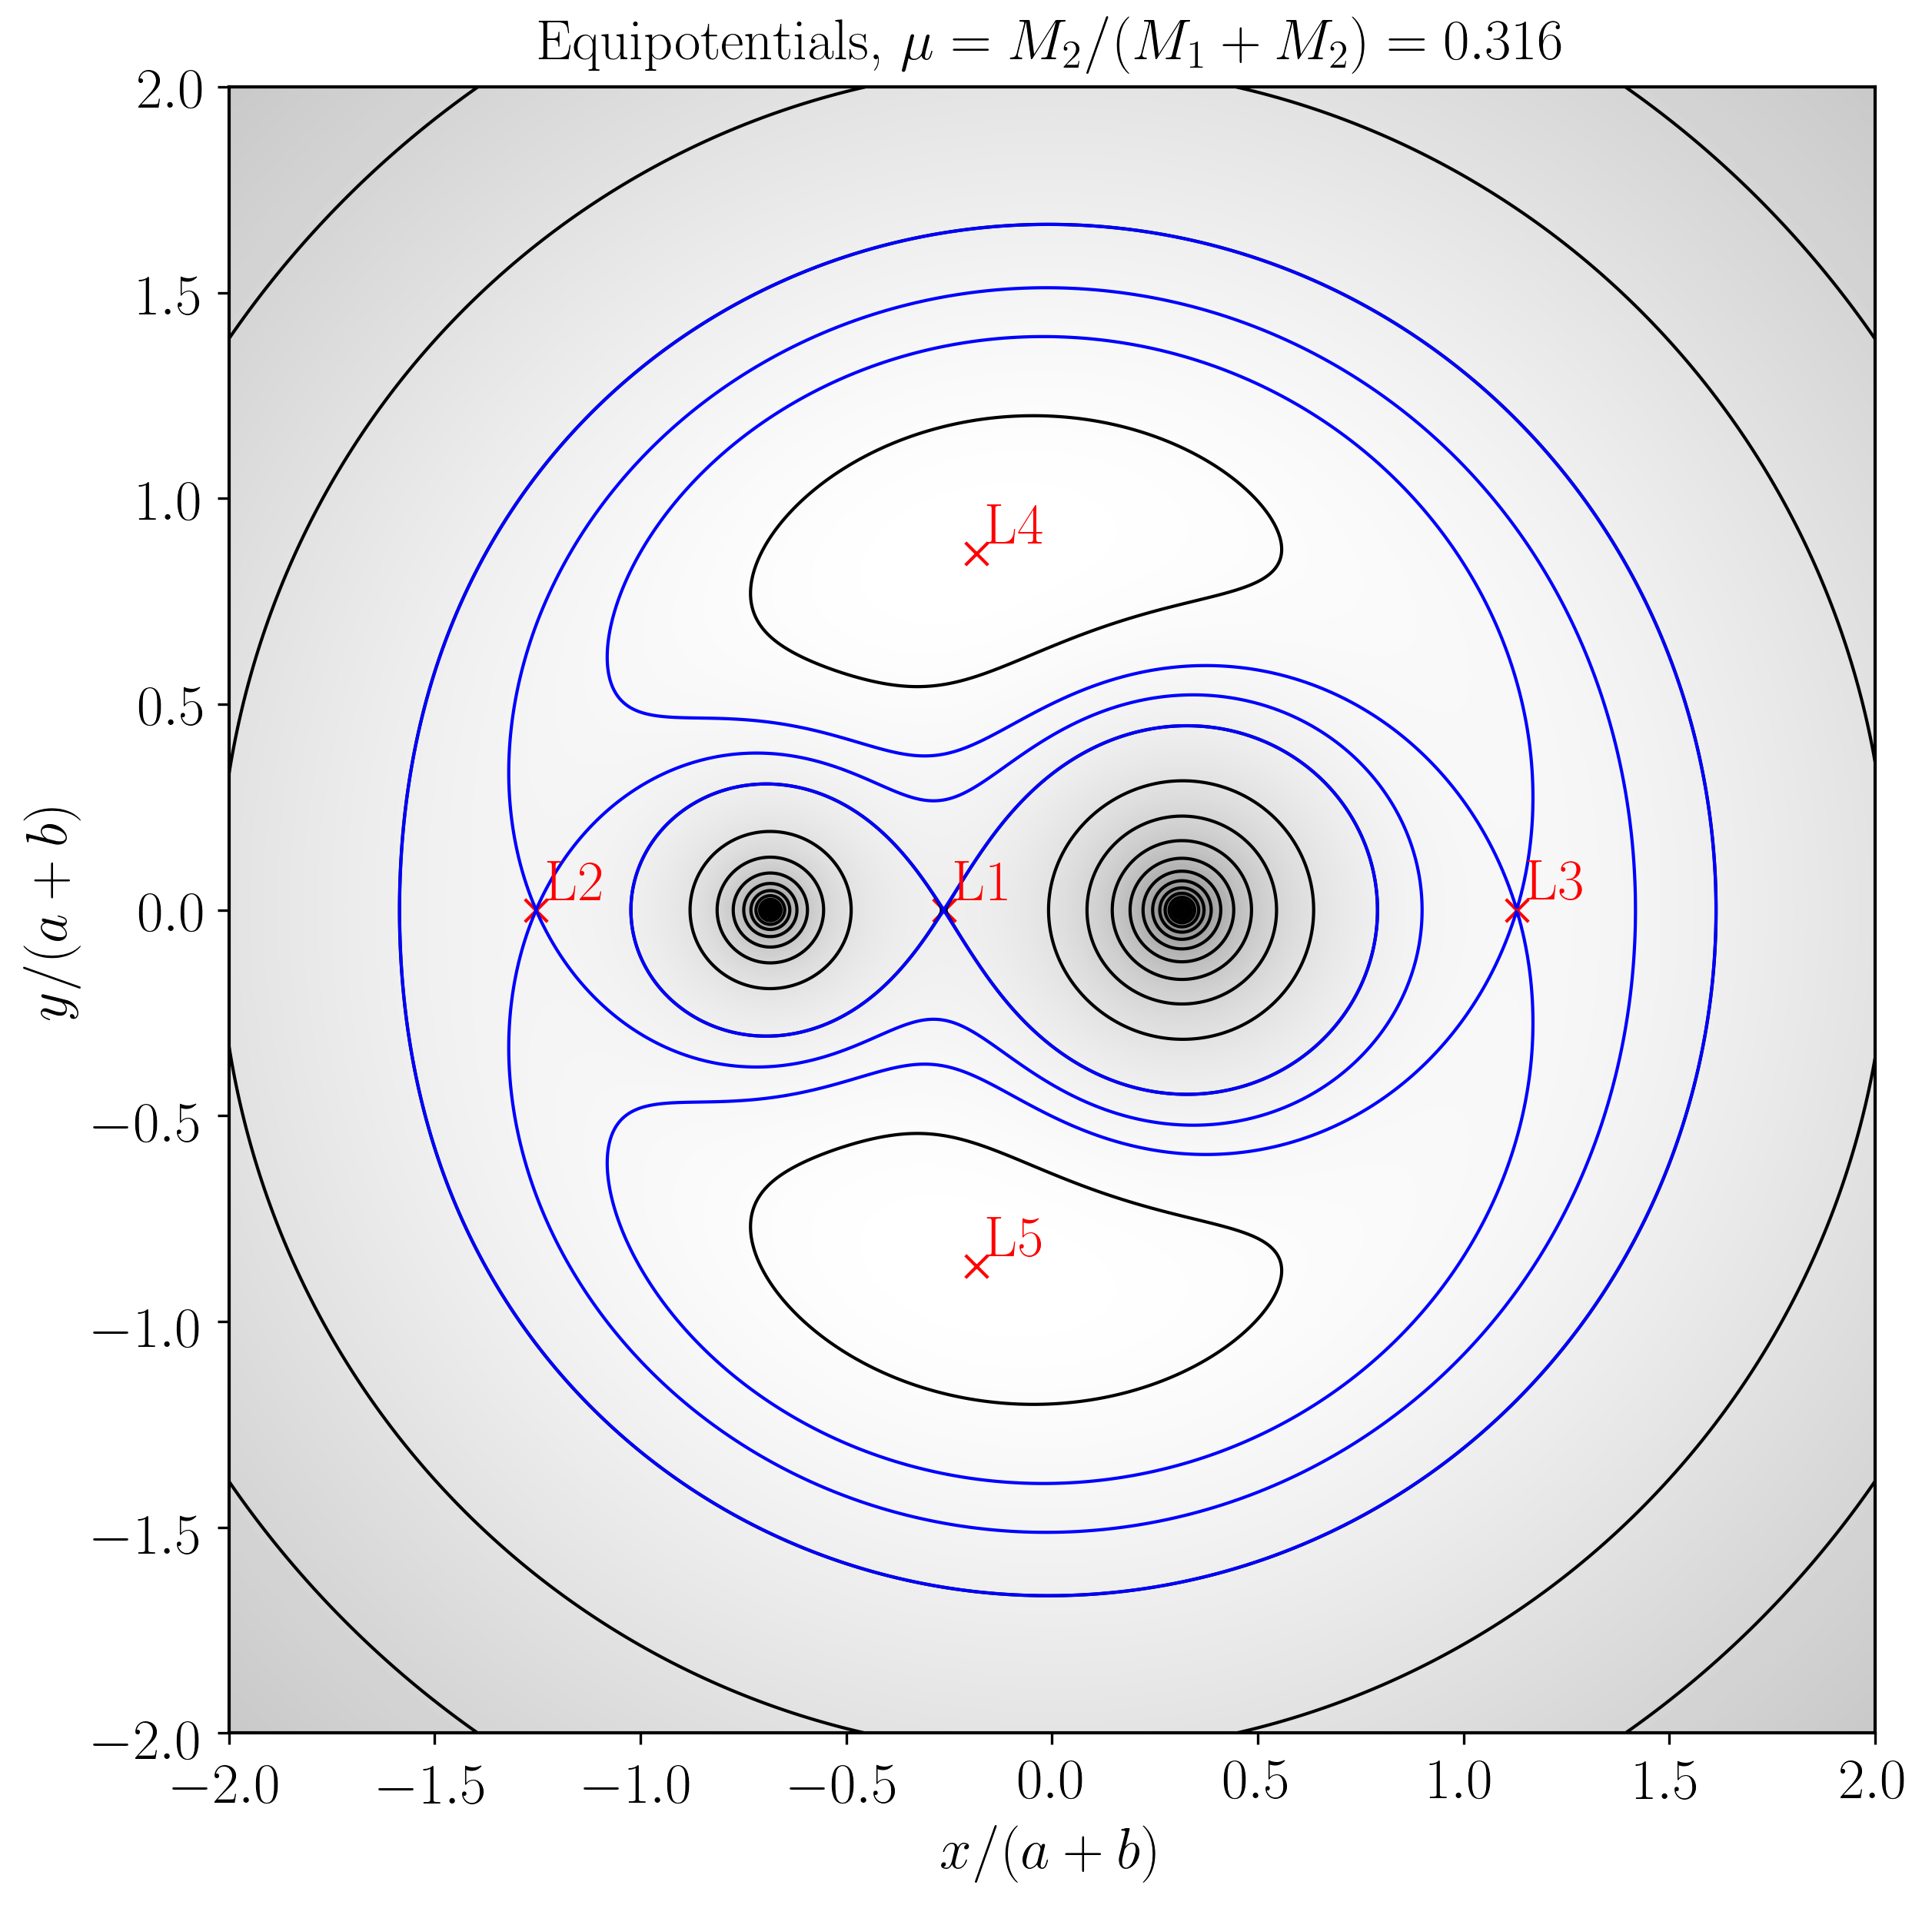
\includegraphics[width = \linewidth]{../figures/chapter1/equipotentials_mu_0_316.png} 
    				\end{subfigure}
    				\hspace{0.01cm}
    				\begin{subfigure}[h]{0.535\textwidth}
        				\centering
        				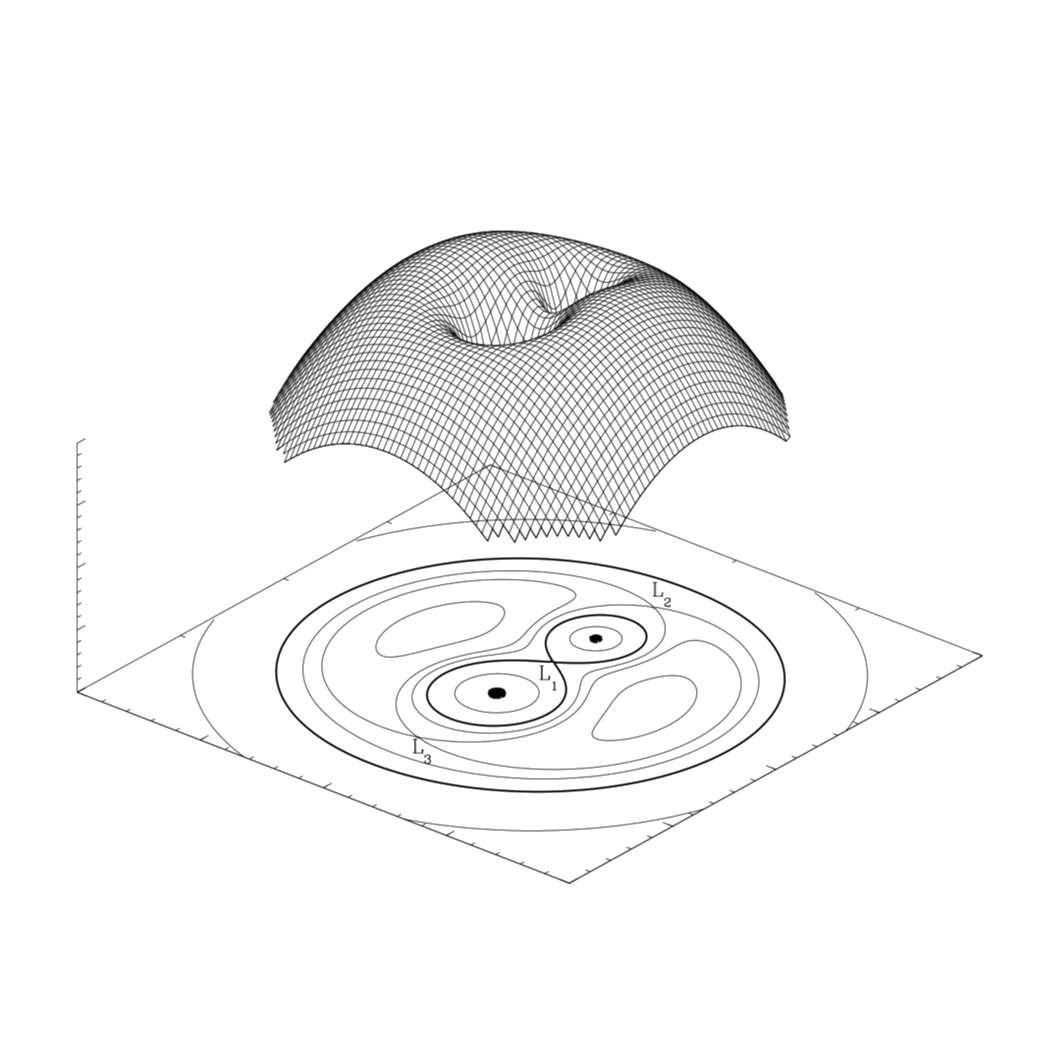
\includegraphics[width = \linewidth]{../figures/chapter1/3Dequipotentials_transparent.png} 
   					 \end{subfigure}
   					 \caption{\textbf{Left panel}: Equipotential lines in the x-y orbital plane of a rotating binary with a reduced mass ratio of $\mu = 0.316$. In this setup, $M_1$ is the more massive and is located at $x = +a$, whilst $M_2$ is the less massive and is at $x = -b$. The inner equipotential surface that passes from the $L_1$ Lagrangian point, defines the "teardrop"-shaped Roche-lobes, one for each star. Contour lines passing through the Lagrange points are marked with blue colour. The image was created based on a \texttt{python} script, courtesy of \cite{Zingale}. \textbf{Right Panel}: 3D representation of equipotential surfaces. The image was adapted from \cite{Sluijs}.}
   					 \label{fig:eq_sur}
				\end{figure}
				
				From the five Lagrangian points, the $L_1$ plays a key role in the evolution of binary systems since the equipotential surface\footnote{An equipotential surface is defined as the collection of all points in the system that share the same value of the effective gravitational potential, $\Phi$.} passing through that inner point, defines the \emph{Roche-lobe}. The shape of the equipotential surfaces is illustrated in \hyperref[fig:eq_sur]{Fig 1.2}; they assume a concentric spherical shape in proximity to the two stars whilst, as a result of the combined gravitational influence of the two masses, they get distorted when we move further away.
				
				During the various evolutionary stages, the star might inflate and increase its radius to such a degree that the volume of the star exceeds the volume defined by its Roche-lobe. This will cause a transfer of surface material from that star to its companion via the $L_1$ point triggered by the unbalanced pressure in that direction; this process is known as \emph{Roche-lobe overflow} (RLOF) and the donor star can lose a substantial amount of its total mass. Unfortunatelly, there is no analytical expression for the size of a Roche-lobe in a given binary. However, \cite{Eggleton1983} has proposed a numerical approximation of the radius of the Roche-lobe given by the following equation
				
				\begin{eqnarray}
					\label{eq:rl_radius}
					\frac{R_L}{\alpha} = \frac{0.49 q^{2/3}}{0.6 q^{2/3} + \ln(1 + q^{1/3})}
				\end{eqnarray}				 
				where $\alpha$ is the orbital separation, and $q \equiv M_{\text{donor}} / M_{\text{accretor}}$ is the mass ratio of the binary components. These are the two most important orbital parameters that we need to know in order to follow the evolution of the binary.
				
				It is maybe worth mentioning that as matter spills across the inner Lagrangian point, it forms an \emph{accretion disk} rather than falling directly onto the companion star. This happens simply because the accreted material possesses the same angular momentum as the donor star, and unless there are non-conservative processes able to remove some of the angular momentum of the accreted gas, it will continue to orbit around the companion star.
				
				Based on which equipotential surfaces are filled, we can classify binary systems into three categories \citep[see also][]{Weigert1968}:
					\begin{enumerate*}[label=(\roman*)]
						\item \emph{detached binaries} where the radii of both stars are much smaller than their orbital separation; neither of the two stars fills its respective Roche-lobe, and they evolve almost independently of each other,
						\item \emph{semi-detached binaries} where only one of the two stars fills its Roche-lobe leading to distortion of the equipotential surfaces from their spherical shape, and mass transfer occurs, and
						\item \emph{contact binaries} where both stars fill their Roche-lobe. This situation results to a shared, common atmosphere that might be ejected, stripping the system from a significant amount of mass.
					\end{enumerate*}									
				

					
			\subsection{Mass transfer}
			
				%Cases A/B/C, (wind mass accretion + Roche lobe overflow) etc		
				From the discussion above, it becomes clear that the mass transfer rate via RLOF and its stability depends on the extent to which the donor star overfills its Roche-lobe. Especially the stability of the mass transfer depends on how the donor star responses to this sudden mass loss; for \emph{stable} mass transfer, the donor must remain within its Roche-lobe \citep[see][for discussion]{Ivanova2015, Postnov2014, Soberman1997, Kalogera1996}.
				
				Based on the evolutionary status of the donor star when it fills its Roche-lobe, we can discern three cases of mass transfer \citep{Kipp1967, Lauterborn1970}:
				
				\begin{enumerate}[label=(\roman*)]
					\item \emph{Case A}: mass transfer commences while the star is still in the MS, i.e. during core hydrogen burning;
					\item \emph{Case B}: the donor star fills its Roche-lobe after the Hygrogen has been depleted from its core but before helium ignition;
					\item \emph{Case C}: refers to RLOF after the exhaustion of helium in the core, and includes all the subsequent stages.
				\end{enumerate}
				For helium stars in particular, we can define the cases \emph{BA}, \emph{BB}, and \emph{BC} for mass transfer during He core burning, He-shell burning, and carbon core burning respectively.
				
				Finally, if the donor star is massive enough, it is likely to experience very strong stellar winds that will remove a considerable amount of mass even without filling its Roche-lobe. A fraction of this mass lost via winds might be accreted by its companion star; this is refered to as \emph{wind mass transfer}, and although it provides a less efficient way to transfer mass, compared to RLOF, it can be important in some binaries.
				
			\subsection{Common envelope}
			
				%Explain a little bit in more detail the basics of CE
				When mass is transfered via RLOF in a dynamically unstable manner, i.e. when the convective envelope of the donor star continues to expand despite the mass loss, the mass loss rate naturally increases. The companion star accretes material stably at its thermal timescale, which is orders of magnitude larger than the dynamical timescale at which the donor star loses mass, thus it grows until it fills its Roche-lobe as well \citep{Izzard_CE}; at this point, the two stars form a contact binary system, and share a common envelope (CE).
				
				Since the orbital plane of the two stars lies within the CE, a drag force will be developed due to friction, caused by the motion of the stars. The system then goes through a \emph{spiral-in} phase, during which a dissipation of orbital angular momentum leads to the decay of the orbit (i.e., a reduction of the orbital separation). This plunge phase occurs on an orbital timescale of a few years \citep{Izzard_CE}, and the energy lost from the orbit is being deposited in the surrounding envelope. The reaction of the envelope to this energy deposition is to expand and potentially ejected from the binary. The ultimate outcome of the CE stage is a more tight binary with a reduced total mass (assuming that the orbital shrinkage during the CE phase didn't result to a merging of the two cores). For this reason, although the physical background of the CE phase described above is still not well understood, it has been hypothized that it plays a crucial role in the formation of a wide variety of binary systems, including double neutron star systems. For a complete review of our current understanding of CE evolution, we refer to the work of \cite{Ivanova_CE}.
				
			\subsection{Angular momentum losses}
			
				%Effects of angular momentum transfer + magnetic braking
				Orbital angular momentum variations, and the mechanisms via which this can occur play an important role in the evolution of a binary since it directly affects the orbital period of the system. Angular momentum can be extracted from a binary system on different timescales \citep{Yakut2008} mainly via the following processes:
				
				\begin{enumerate}[label=(\roman*)]
				
					\item \emph{Non-conservative mass transfer}: If during mass transfer, the companion star accretes only a fraction of the mass lost from the donor, the rest will carry away some of the specific angular momentum.
					\item \emph{Magnetic braking}: As it was mentioned above, the differential rotation of stars is responsible for the production of magnetic fields and, subsequently, magnetized stellar winds. Interactions with the magnetic fields can give raise to tidal effects, causing a rotating star to sync and corotate with the orbit (tidally locked system). If the spin of the star is originally larger than the orbital period, this is essentially translated to angular momentum removal from the binary \citep[see also][]{Rappaport1983}.
					\item \emph{Gravitational waves}:  These are perturbations of the space-time manifold caused by various kinds of motion and asymmetric distribution of masses in a close binary. Like classical waves, gravitational waves carry energy (often dubbed as gravitational radiation) that is being lost from the system causing the angular momentum to decrease and the orbit to shrink \citep[see also][]{Peters1964, Riles2013}.
				
				\end{enumerate}
				
				
			\subsection{Double neutron star systems}
			
				Since the aim of this thesis is to investigate the connection between progenitor and remnant masses in double neutron star (DNS) binaries, it is considered appropriate to devote a subsection on the formation and the importance of these incredible systems.
				
				Initially massive binaries which their components are close enough to interact with each other, will undergo several stages that are plagued with uncertainties before they end up as neutron stars. The most acceptable scenario for the formation of DNS systems up to this date begins with the evolution of the more massive (primary) component, which naturally happens on a shorter timescale than its companion. The primary star will fill its Roche-lobe transferring material to the companion star and exposing its helium core. Further evolution of the newly formed He-star will lead to a supernova explosion which could unbound the whole system. 
				
				If the binary survives the explosion, the first-born neutron star can be detected as a radio pulsar orbiting a massive main sequence star (OB-star). As the latter evolves, mass transfer will be initiated and the system can be observed as a high-mass X-ray binary (HMXB) due to the accelerated infalling material onto the surface of the neutron star. When the secondary star expands to a degree that can engulf the neutron star, a common envelope is formed; assuming that during the spiral-in phase a coalescence of the two stars will not occur, a binary system consisting of a neutron star and a helium star will emerge.
				
				Depending on the mass of the He-star, its evolutionary stage, and the orbital separation of the two components, a second mass transfer event may occur stripping the donor star from its helium-rich envelope and spinning up the accreting neutron star. The neutron star that has been spun up during this process is often dubbed \emph{recycled} and is believed to be the origin of millisecond pulsars.
				
				Finally, the second neutron star will be formed in a low-energy supernova (see below). The final fate of such systems, depending on the post-SN orbital separation and eccentricity of the binary, is to merge due to gravitational waves damping. The remnant -if any- that is left behind from such an event is most likely a single black hole. All the stages leading to the formation of DNS binaries that were described above are presented in \hyperref[fig:DNS]{Fig 1.3} and exhaustively discussed in the work of \cite{Tauris2017}.
				
				\begin{figure}[h]
					\centering
					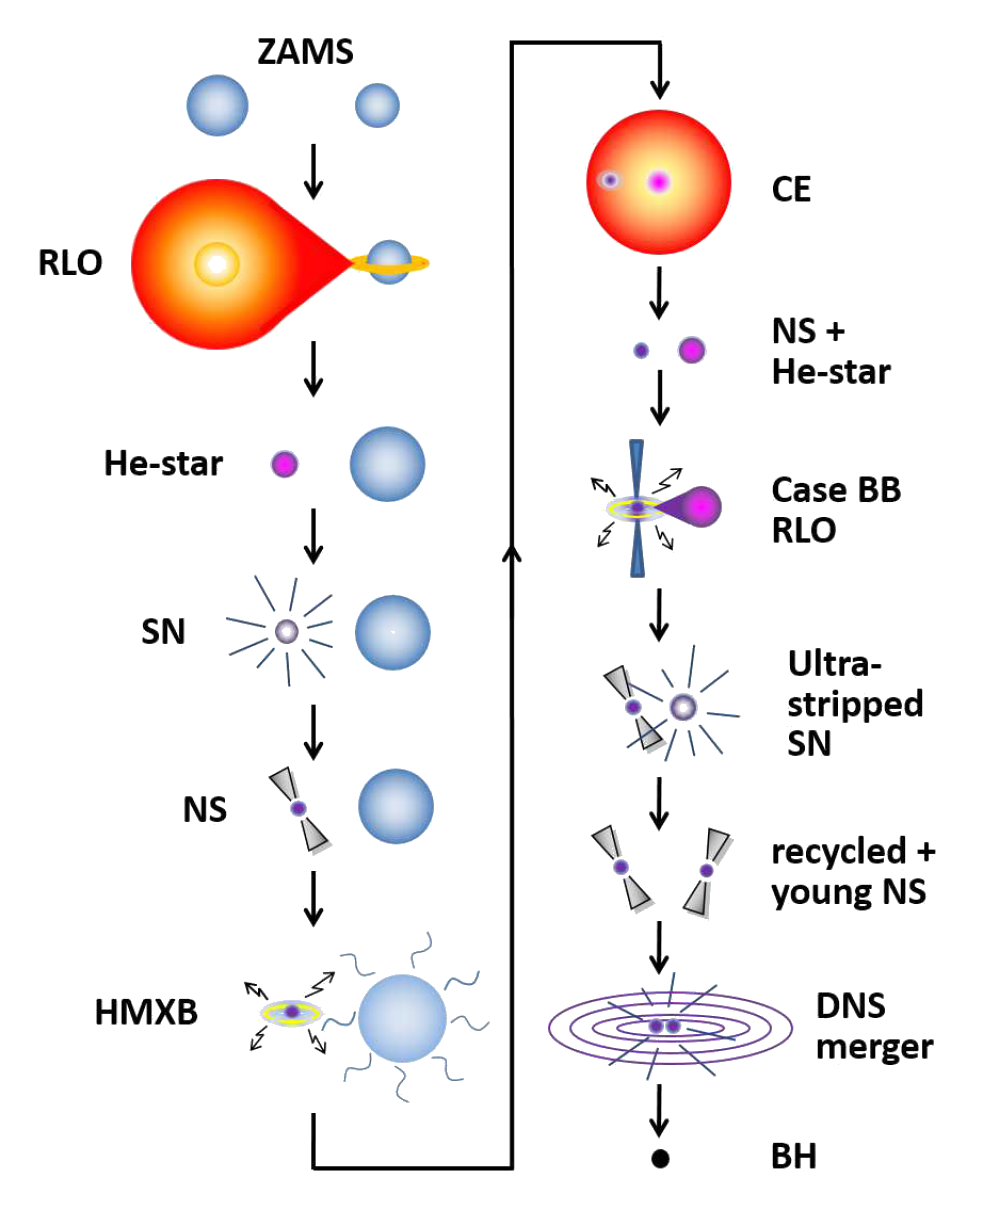
\includegraphics[scale = 0.85]{../figures/chapter1/DNS_formation_transparent.png}
					\caption{Illustration of the formation of a DNS system which merges within a Hubble time and produces a single black hole. Image and caption taken from \cite{Tauris2017}.}
					\label{fig:DNS}
				\end{figure}
				
				Double neutron star binaries are remarkable systems and excellent sources of gravitational waves. This enables them to act as probes and shed some light on all the uncertain evolutionary stages that lead to their formation, e.g. CE evolution, nature and asymmetries of SNe explosions, velocity kicks imparted onto newborn neutron stars as well as their mass distribution. For a more complete coverage see \cite[][and references therein]{Tauris2017, Ivanova_DNS, Dewi_DNS}.
				
	\section{Stellar transients}
	
		%Couple of words for the different types of stellar transients and how can we observe them
		Transient stars are defined as objects which experience a strong variation in their brightness, that can be observed within a human lifetime, due to various instabilities ranging from magnetic-powered flares in small, dim red dwarfs (M-dwarfs) to thermonuclear shell/core flashes, and gravitational collapse of iron cores. Transients can be non-periodic and/or non-recurring events depending on the nature of the underlying instability. Generally, unstable processes like magnetic reconnection, accretion instabilities, and shell flashes have a tendency not to disrupt the star so they might occur a number of times during the lifetime of the star. On the other hand, known disruptions include supernovae and merging events. Here we will briefly discuss the latter scenario of explosive transients.
		
			\subsection{Types of Supernovae}
			
				%Explain in details the difference between core collapse SNe and type Ia and different subdivision
				Massive stars will end their short lives in an extremely luminous supernova (SN) explosion leaving behind a compact object which is either a neutron star or a black hole, depending on the initial mass of the progenitor star, and enriching their host galaxy with all the elements they forged during their lifetime. Classification of supernovae has been traditionally done by their observational characteristics like spectral features, and properties of their light curves as seen in \hyperref[fig:SNe_classification]{Fig 1.4} \citep[see][]{Filippenko1997, Turatto2003}. 
				
				\begin{figure}[h]
					\centering
					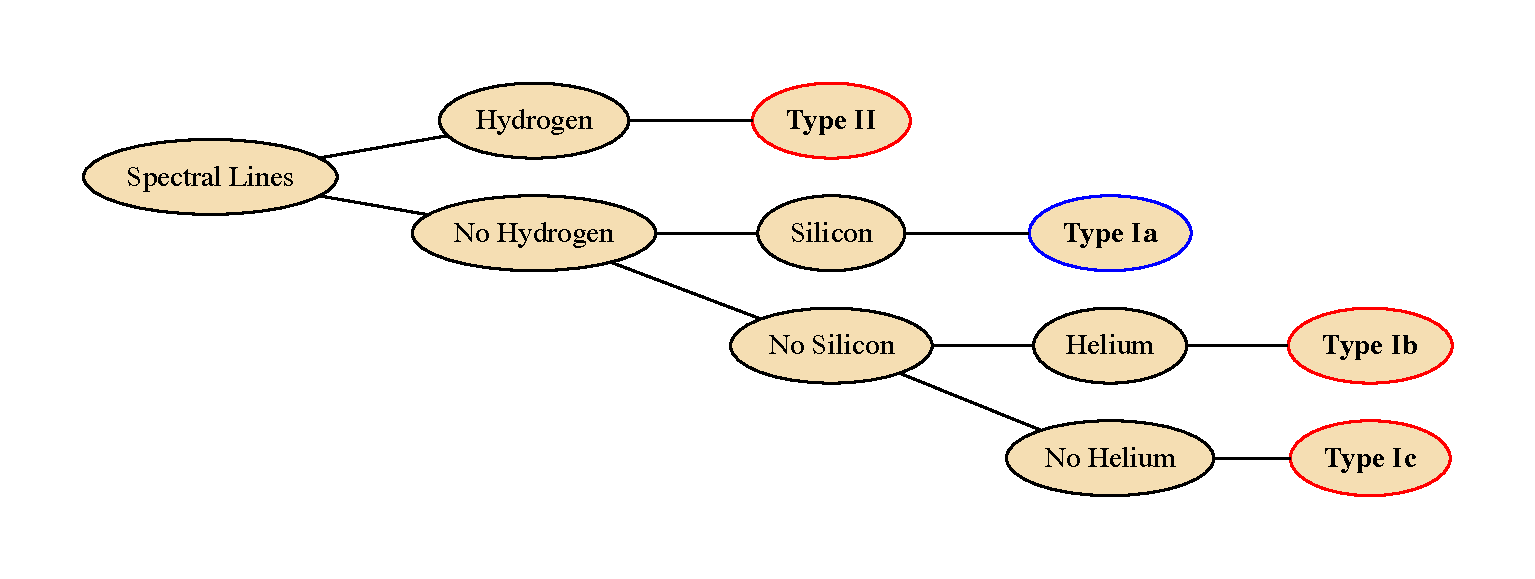
\includegraphics[width = \textwidth]{../figures/chapter1/SNeClass.pdf}
					\caption{Basic classification of supernovae based on their spectra lines. Further sub-groups can be identified if we take into consideration the behavior of their light curves. Type Ia (here marked with a blue circle) is associated with thermonuclear runaway reactions rather than core collapse (red circles).}
					\label{fig:SNe_classification}
				\end{figure}
				
				Whilst there are many physical mechanisms that could potentially lead to a supernova, the connection between the progenitor of the explosion and the type of supernova we eventually observe is still unclear. However, we can differentiate between core collapse SNe (CCSNe) where pressure support is being removed from the core of the star via numerous processes, and thermonuclear explosions of mass-accreting white dwarfs. We will not discuss here the latter case, the associated exploding mechanisms, or how it is related to the type-Ia but the interested reader can refer to the work of \cite{Hillebrandt2000, Wang2018, SNe_book}.
				
				For the case of a star that experiences a gravitational core collapse, there are several channels via which pressure support could be removed from the core; next, we discuss a few aspects of these channels and -to a certain degree- the underlying exploding mechanism.
				
				\subsubsection{Iron core collapse SNe (Fe-CCSNe)}
					
					During the final stages of evolution, if the star is massive enough it will develop an inert iron core. As temperature increases in the core, the energy of the photons becomes sufficiently high to start photodisintegration on the $^{56}$Fe nuclei. This process removes pressure from the core, forcing it to contract until electrons and protons fuse together in a process called \emph{neutronization}. As in all weak interactions, neutronization is accompanied by the production of neutrinos that do not contribute to the pressure support against gravity since they escape the star much faster than photons, and effectively acts as a cooling mechanism carrying energy away. Depending on the mass of the core, the degeneracy pressure provided by the neutrons might be sufficient to cease the collapse leading to the formation of a neutron star. 
					
					Following \cite{Muller2016}, the infalling material will bounce on the surface of the neutron star sending back a shock wave that quickly stalls due to photodisintegration of heavy nuclei and neutrino losses; this is the \emph{pre-explosion phase} and it becomes clear that another energy source is needed in order to have a successful explosion. This source is believed to be a (gain) region behind of the shock where energy deposition of neutrinos leads to heating. The shock revival occurs once the accreted material spends sufficient time in the gain region to receive enough energy from neutrinos to negate its binding energy; the shock is re-energized by the radiation and expands outwards again. At this point we have entered the \emph{explosion phase}. In the case of a very massive core, degeneracy pressure from neutrons is not enough to balance the gravitational pressure, therefore the star will continue to collapse forming a stellar mass black hole. More on the progenitors of CCSNe and relevant exploding mechanisms can be found in \cite{Smartt2009, Couch2017}.

				\subsubsection{Electron capture SNe (ECSNe)}
				
					Formation of an iron core is not the only way to remove pressure support. Less massive stars will form a degenerate ONeMg core where the pressure is provided by the degenerate electrons. If the degenerate core reaches a critical mass of $M^{\text{EC}}_{\text{crit}} = 1.37$ M$_{\odot}$ \citep{Nomoto1984}, electron captures on $^{24}$Mg and $^{20}$Ne nuclei will reduce the number of electrons, and thus the pressure against gravitational contraction, triggering the collapse of the core. The energy released from the electron captures will eventually lead to an oxygen deflagration\footnote{A deflagration process refers to a subsonic front that propagates via thermal conduction as opposed to a detonation process where a supersonic burning front is driven by shock waves.}. However, since oxygen is ignited in a highly degenerate environment there will be no expansion as a response to the temperature increase, as in the case of non-degenerate matter; instead, this increase of temperature will accelerate the rate of fusion and, consequently, the temperature will again increase in a runaway process. The contraction of the core, due to loss of pressure support, increases the density and leads to more rapid electron captures, at a rate that can overcome the oxygen deflagration and continue to collapse up to neutron star density.
					
					The core is believed to collapse more rapidly than in the case of Fe-CCSNe, launching a shock wave in accordance with core bounce and subsequent neutrino heating as explained above. The final result is a dim supernova with a relatively low explosion energy and low $^{56}$Ni ejecta mass \citep{Jones2016}. Two-dimensional simulations have shown that the explosion exhibit almost spherical symmetry \citep{Nomoto2014} since the rapid nature of the explosion leave less time for asymmetries to develop \citep{Jones2016}, thus ECSNe do not impart large natal velocity kicks to the newly-formed neutron star.
					
					The late evolutionary stages of these lower-mass stars are riddled with uncertainties resulting to a very narrow mass-range for the progenitors of ECSNe. To complicate things even more, if these stars are part of a binary system, interactions between the two stars can give raise to new channels for ECSNe to emerge. For this case, we refer to \cite{Siess2018, Giacobbo2018, Poelarends2017}.
 				
				\subsubsection{Pair instability SNe (PISNe)}
				
					So far we discussed the final fate of massive stars that develop an iron core, and the less certain evolution of lower-mass stars that develop a degenerate ONeMg core. At the opposite end we find the case of very massive stars, i.e. stars with initial mass $M_{\text{init}} > 100$ M$_{\odot}$. It has been suggested \citep{langer12} that these enormous stars undergo a dynamical collapse before core oxygen ignition, caused by electron-positron pair creation that effectively reduces the radiation pressure in the stellar core, leaving behind no remnant. PISNe are expected to produce a wide variety of SN types depending on their mass range \citep{Gilmer2017}. We will not discuss further this particular branch of SNe since it poses no interest for this thesis. For this reason, the inquisitive reader is referred to the work of \cite{Langer_PISNe, Woosley_PISNe, Kozyreva2017, Gilmer2017}.
					
				
				
			\subsection{Type Ib/c Supernovae}
			
				%Explain in details this particular branch + ultra stripped SNe
				Supernova explosions of naked helium stars are expected to be observed as Type Ib or Type Ic due to their lack of a hydrogen mantle \hyperref[fig:SNe_classification]{(Fig 1.4)}. Additionally, in order to be classified as Type Ic, the progenitor star must be also stripped from its helium envelope\footnote{There is a caveat in this formulation; helium can be detected only if it has been excited by the radioactive decay of $^{56}$Ni. If a substantial amount of He is present after the explosion but -somehow- shielded from $^{56}$Ni, the SN would be still classified (falsely) as Type Ic! The amount of synthesized $^{56}$Ni along with the efficiently mixing into the He-envelope remains crucial for that matter.} either via strong stellar winds or binary interactions. As \cite{Yoon2010} mention, population studies indicate that the majority of SNe Ib/c are produced in binary systems without the need of single star progenitors in order to match their observed rate. This can be important since the nature of the explosion will determine if the binary shall remain bound after the explosion or break apart into two loose components.
				
				Of particular interest for this thesis is the case of \emph{ultra-stripped} SNe as described in \cite{Tauris_ultra, Tauris2013}. The authors showed that a helium star can be heavily stripped as a result of the binary interaction with a neutron star, ultimately leading to a very faint SN-Ic with a mass ejecta of only $\lesssim 0.2$ M$_{\odot}$. The implication of such small amount of ejecta can be quite important in the formation of DNS systems since the binding energy of the envelopes is expected to be smaller than the one found in normal SNe, imparting only a small kick in the second neutron star.
				
				For an overview of the expected light curve properties of ultra-stripped SNe, see \cite{Moriya2017}.
				
				
    \end{document}
    